% Options for packages loaded elsewhere
\PassOptionsToPackage{unicode}{hyperref}
\PassOptionsToPackage{hyphens}{url}
%
\documentclass[
]{article}
\usepackage{amsmath,amssymb}
\usepackage{lmodern}
\usepackage{iftex}
\ifPDFTeX
  \usepackage[T1]{fontenc}
  \usepackage[utf8]{inputenc}
  \usepackage{textcomp} % provide euro and other symbols
\else % if luatex or xetex
  \usepackage{unicode-math}
  \defaultfontfeatures{Scale=MatchLowercase}
  \defaultfontfeatures[\rmfamily]{Ligatures=TeX,Scale=1}
\fi
% Use upquote if available, for straight quotes in verbatim environments
\IfFileExists{upquote.sty}{\usepackage{upquote}}{}
\IfFileExists{microtype.sty}{% use microtype if available
  \usepackage[]{microtype}
  \UseMicrotypeSet[protrusion]{basicmath} % disable protrusion for tt fonts
}{}
\makeatletter
\@ifundefined{KOMAClassName}{% if non-KOMA class
  \IfFileExists{parskip.sty}{%
    \usepackage{parskip}
  }{% else
    \setlength{\parindent}{0pt}
    \setlength{\parskip}{6pt plus 2pt minus 1pt}}
}{% if KOMA class
  \KOMAoptions{parskip=half}}
\makeatother
\usepackage{xcolor}
\usepackage[margin=1in]{geometry}
\usepackage{color}
\usepackage{fancyvrb}
\newcommand{\VerbBar}{|}
\newcommand{\VERB}{\Verb[commandchars=\\\{\}]}
\DefineVerbatimEnvironment{Highlighting}{Verbatim}{commandchars=\\\{\}}
% Add ',fontsize=\small' for more characters per line
\usepackage{framed}
\definecolor{shadecolor}{RGB}{248,248,248}
\newenvironment{Shaded}{\begin{snugshade}}{\end{snugshade}}
\newcommand{\AlertTok}[1]{\textcolor[rgb]{0.94,0.16,0.16}{#1}}
\newcommand{\AnnotationTok}[1]{\textcolor[rgb]{0.56,0.35,0.01}{\textbf{\textit{#1}}}}
\newcommand{\AttributeTok}[1]{\textcolor[rgb]{0.77,0.63,0.00}{#1}}
\newcommand{\BaseNTok}[1]{\textcolor[rgb]{0.00,0.00,0.81}{#1}}
\newcommand{\BuiltInTok}[1]{#1}
\newcommand{\CharTok}[1]{\textcolor[rgb]{0.31,0.60,0.02}{#1}}
\newcommand{\CommentTok}[1]{\textcolor[rgb]{0.56,0.35,0.01}{\textit{#1}}}
\newcommand{\CommentVarTok}[1]{\textcolor[rgb]{0.56,0.35,0.01}{\textbf{\textit{#1}}}}
\newcommand{\ConstantTok}[1]{\textcolor[rgb]{0.00,0.00,0.00}{#1}}
\newcommand{\ControlFlowTok}[1]{\textcolor[rgb]{0.13,0.29,0.53}{\textbf{#1}}}
\newcommand{\DataTypeTok}[1]{\textcolor[rgb]{0.13,0.29,0.53}{#1}}
\newcommand{\DecValTok}[1]{\textcolor[rgb]{0.00,0.00,0.81}{#1}}
\newcommand{\DocumentationTok}[1]{\textcolor[rgb]{0.56,0.35,0.01}{\textbf{\textit{#1}}}}
\newcommand{\ErrorTok}[1]{\textcolor[rgb]{0.64,0.00,0.00}{\textbf{#1}}}
\newcommand{\ExtensionTok}[1]{#1}
\newcommand{\FloatTok}[1]{\textcolor[rgb]{0.00,0.00,0.81}{#1}}
\newcommand{\FunctionTok}[1]{\textcolor[rgb]{0.00,0.00,0.00}{#1}}
\newcommand{\ImportTok}[1]{#1}
\newcommand{\InformationTok}[1]{\textcolor[rgb]{0.56,0.35,0.01}{\textbf{\textit{#1}}}}
\newcommand{\KeywordTok}[1]{\textcolor[rgb]{0.13,0.29,0.53}{\textbf{#1}}}
\newcommand{\NormalTok}[1]{#1}
\newcommand{\OperatorTok}[1]{\textcolor[rgb]{0.81,0.36,0.00}{\textbf{#1}}}
\newcommand{\OtherTok}[1]{\textcolor[rgb]{0.56,0.35,0.01}{#1}}
\newcommand{\PreprocessorTok}[1]{\textcolor[rgb]{0.56,0.35,0.01}{\textit{#1}}}
\newcommand{\RegionMarkerTok}[1]{#1}
\newcommand{\SpecialCharTok}[1]{\textcolor[rgb]{0.00,0.00,0.00}{#1}}
\newcommand{\SpecialStringTok}[1]{\textcolor[rgb]{0.31,0.60,0.02}{#1}}
\newcommand{\StringTok}[1]{\textcolor[rgb]{0.31,0.60,0.02}{#1}}
\newcommand{\VariableTok}[1]{\textcolor[rgb]{0.00,0.00,0.00}{#1}}
\newcommand{\VerbatimStringTok}[1]{\textcolor[rgb]{0.31,0.60,0.02}{#1}}
\newcommand{\WarningTok}[1]{\textcolor[rgb]{0.56,0.35,0.01}{\textbf{\textit{#1}}}}
\usepackage{longtable,booktabs,array}
\usepackage{calc} % for calculating minipage widths
% Correct order of tables after \paragraph or \subparagraph
\usepackage{etoolbox}
\makeatletter
\patchcmd\longtable{\par}{\if@noskipsec\mbox{}\fi\par}{}{}
\makeatother
% Allow footnotes in longtable head/foot
\IfFileExists{footnotehyper.sty}{\usepackage{footnotehyper}}{\usepackage{footnote}}
\makesavenoteenv{longtable}
\usepackage{graphicx}
\makeatletter
\def\maxwidth{\ifdim\Gin@nat@width>\linewidth\linewidth\else\Gin@nat@width\fi}
\def\maxheight{\ifdim\Gin@nat@height>\textheight\textheight\else\Gin@nat@height\fi}
\makeatother
% Scale images if necessary, so that they will not overflow the page
% margins by default, and it is still possible to overwrite the defaults
% using explicit options in \includegraphics[width, height, ...]{}
\setkeys{Gin}{width=\maxwidth,height=\maxheight,keepaspectratio}
% Set default figure placement to htbp
\makeatletter
\def\fps@figure{htbp}
\makeatother
\setlength{\emergencystretch}{3em} % prevent overfull lines
\providecommand{\tightlist}{%
  \setlength{\itemsep}{0pt}\setlength{\parskip}{0pt}}
\setcounter{secnumdepth}{-\maxdimen} % remove section numbering
\ifLuaTeX
  \usepackage{selnolig}  % disable illegal ligatures
\fi
\IfFileExists{bookmark.sty}{\usepackage{bookmark}}{\usepackage{hyperref}}
\IfFileExists{xurl.sty}{\usepackage{xurl}}{} % add URL line breaks if available
\urlstyle{same} % disable monospaced font for URLs
\hypersetup{
  pdftitle={Seance 5: Paramètres de dispersion},
  pdfauthor={Visseho Adjiwanou ; Sociology department, Université du Québec à Montréal (UQAM); co-authors; },
  hidelinks,
  pdfcreator={LaTeX via pandoc}}

\title{Seance 5: Paramètres de dispersion}
\author{Visseho Adjiwanou \footnote{corresponding author -
  \href{mailto:adjiwanou.vissého@uqam.ca}{\nolinkurl{adjiwanou.vissého@uqam.ca}}} \and Sociology
department, Université du Québec à Montréal
(UQAM) \and co-authors \and }
\date{31 January 2023}

\begin{document}
\maketitle

\hypertarget{plan-de-pruxe9sentation}{%
\subsection{Plan de présentation}\label{plan-de-pruxe9sentation}}

\begin{itemize}
\item
  Mesures
\item
  Extension

  \begin{itemize}
  \tightlist
  \item
    Scores standardisés ou scores-Z
  \item
    Loi normale
  \item
    Distribution d'échantillonnage
  \item
    Théorème central limite
  \item
    Intervalles de confiances
  \end{itemize}
\end{itemize}

\hypertarget{introduction}{%
\subsection{Introduction}\label{introduction}}

\begin{itemize}
\tightlist
\item
  Bien que la moyenne soit la caractéristique la plus importante
  résumant une distribution à l'aide d'un seul nombre, il est nécessaire
  aussi d'étudier comment les observations sont dispersées, ou variées.
\end{itemize}

\begin{quote}
\begin{itemize}
\tightlist
\item
  On donne l'exemple d'homme qui s'est noyé dans un ruisseau qui avait
  en moyenne 10 centimètres de profondeur
\end{itemize}
\end{quote}

\begin{quote}
\begin{itemize}
\tightlist
\item
  De même qu'il existe différentes mesures de valeur centrale, on trouve
  de nombreuses mesures de la dispersion.
\end{itemize}
\end{quote}

\begin{quote}
\begin{itemize}
\tightlist
\item
  deux d'entre elles sont généralement utilisées:
\item
  l'\textbf{intervalle interquartile} et
\item
  l'\textbf{écart type}
\end{itemize}
\end{quote}

\begin{quote}
\begin{itemize}
\tightlist
\item
  Nous en citerons d'autres tout au long de la présentation
\end{itemize}
\end{quote}

\hypertarget{uxe9tendue}{%
\subsection{Étendue}\label{uxe9tendue}}

\begin{itemize}
\item
  L'\textbf{étendue} (ou \emph{range} ou \emph{amplitude}) est
  simplement la différence entre la plus grande et la plus petite valeur
  de la variable.
\item
  Étendue = plus grande observation - plus petite observation
\end{itemize}

\hypertarget{uxe9tendue-interquartile-eiq}{%
\subsection{Étendue Interquartile
(EIQ)}\label{uxe9tendue-interquartile-eiq}}

\begin{itemize}
\item
  Au lieu d'utiliser les deux observations extrêmes, prenons les deux
  quartiles.
\item
  les deux quartiles sont beaucoup plus stables (i.e.~stables à
  l'influence indue d'une seule observation).
\item
  La distance séparant les quartiles mesure la dispersion de la moitié
  centrale des observations: c'est pourquoi on l'appelle \textbf{étendue
  interquartile (EID)}, ou \textbf{dispersion centrale}.
\item
  EIQ = 3ème quartile - 1er quartile
\item
  Limite: Elle n'utilise pas l'ensemble des observations de la
  distribution.
\end{itemize}

\hypertarget{variance}{%
\subsection{Variance}\label{variance}}

\begin{itemize}
\tightlist
\item
  La \textbf{variance} est la moyenne arithmétique des carrés des écarts
  à la moyenne
\item
  Elle mesure la dispersion, l'étalement, et la variabilité des valeurs
\item
  Pour une distribution, la variance est:
\end{itemize}

\[Variance = s^2 = \frac{1}{n-1} \sum_{i=1}^n (X_i - \bar{X})^2\]

\[s^2 = \frac{1}{n-1} *[(X_1 - \bar{X})^2 + (X_2 - \bar{X})^2 + ... + (X_n - \bar{X})^2]\]

\begin{itemize}
\tightlist
\item
  \(X_1, X_2, ... , X_n\) sont les n valeurs observées et \(\bar{X}\) =
  moyenne de la distribution
\end{itemize}

\hypertarget{variance-1}{%
\subsection{Variance}\label{variance-1}}

\begin{itemize}
\tightlist
\item
  Pour les données classées, il faut modifier cette formule, en
  pondérant chaque écart par sa fréquence.
\end{itemize}

\[Variance, s^2 = \frac{1}{n-1} \sum_{i=1}^p f_i(x_i - \bar{x})^2\]

\begin{itemize}
\item
  \(x_1, x_2, ... , x_p\) étant les p occurrences observées avec
  \(n_1, n_2, ... , n_p\), les effectifs correspondants de ces
  occurrences.
\item
  \(f_1, f_2, ... , f_p\) sont les fréquences relatives et \(\bar{x}\) =
  moyenne de la distribution groupée (classée)
\end{itemize}

\hypertarget{variance-2}{%
\subsection{Variance}\label{variance-2}}

\begin{itemize}
\tightlist
\item
  la variance est elle aussi très sensible aux valeurs extrêmes
\item
  soit la série de 9 valeurs suivantes : 1, 2, 3, 4, 6, 5, 9, 7, 2.
\item
  on trouve :
\item
  moyenne = 4,3 et variance = 7
\item
  si la valeur 9 est plutôt 90, alors la moyenne = 14,1 et la variance =
  816,1
\end{itemize}

\hypertarget{autres-exemples}{%
\subsection{Autres exemples}\label{autres-exemples}}

\begin{longtable}[]{@{}lll@{}}
\toprule()
Groupe A: & Groupe B & Groupe C \\
\midrule()
\endhead
Relativement homogène & Entre les deux & Relativement hétérogènes \\
\bottomrule()
\end{longtable}

64 44 34 68 63 58 70 80 90 71 91 101 69 74 79 66 56 46 \textbf{68}
\textbf{68} \textbf{68}

\begin{itemize}
\tightlist
\item
  En gras, moyenne de chaque groupe
\end{itemize}

\hypertarget{uxe9cart-type}{%
\subsection{Écart type}\label{uxe9cart-type}}

\begin{itemize}
\item
  Pour éliminer le fait d'avoir utilisé le carré des écarts, on calcule
  finalement la racine carrée de la variance: ceci donne la façon la
  plus générale de mesurer l'écart par rapport à la moyenne, appelée
  pour cette raison son écart type \textbf{s}
\item
  \textbf{écart-type} = racine carrée de la \textbf{variance}
\end{itemize}

\hypertarget{en-ruxe9sumuxe9-mesure-de-tendance-centrale-paramuxe8tres-de-position}{%
\subsection{En résumé : Mesure de tendance centrale (paramètres de
position)}\label{en-ruxe9sumuxe9-mesure-de-tendance-centrale-paramuxe8tres-de-position}}

\begin{longtable}[]{@{}lll@{}}
\toprule()
Symbole & Définition & Formules \\
\midrule()
\endhead
Moyenne & Somme des valeurs divisée par &
\(\bar{X} = \frac{1}{n} \sum_{i=1}^n X_i\) \\
& l'effectif de la série & \\
Médiane & Valeur qui divise la distribution & \\
& en deux parties égales & \\
Mode & Valeur observée de fréquence maximum & \\
Percentile & Valeurs qui divisent la distribution & \\
& en 100 parties égales & \\
\bottomrule()
\end{longtable}

\hypertarget{en-ruxe9sumuxe9-mesure-de-dispersion}{%
\subsection{En résumé : Mesure de
dispersion}\label{en-ruxe9sumuxe9-mesure-de-dispersion}}

\begin{longtable}[]{@{}lll@{}}
\toprule()
Symbole & Définition & Formules \\
\midrule()
\endhead
Étendue & Différence entre la plus grande & G - P \\
& et la plus petite valeur de la & \\
& variable & \\
EIQ & 3ème quartile - 1er quartile & Q3 - Q1 \\
Déviation & La distance d'une valeur à & \(X - \bar{X}\) \\
& la moyenne & \\
Sommes & Somme des carrés des déviations & SC =
\(\sum_{i=1}^n (X_i - \bar{X})^2\) \\
des carrés & & \\
Variance & Moyenne des carrés des déviances &
\(s^2 = \frac{1}{n-1} \sum_{i=1}^n (X_i - \bar{X})^2\) \\
Écart-type & Racine carrée de la variance &
\(s = \sqrt{\frac{1}{n-1} \sum_{i=1}^n (X_i - \bar{X})^2}\) \\
\bottomrule()
\end{longtable}

\hypertarget{scores-standardisuxe9s-ou-scores-z}{%
\subsection{Scores standardisés ou
scores-Z}\label{scores-standardisuxe9s-ou-scores-z}}

\begin{itemize}
\tightlist
\item
  Un score standardisé mesure à combien d'écarts-types de la moyenne se
  situe un score donné
\item
  Sa formule est :
\end{itemize}

\[Z_i = \frac{X_i - \bar{X}}{s}\]

\begin{itemize}
\item
  \(Z_i\) = le score standadisé du \(i^e\) cas
\item
  \(X_i\) = le score du \(i^e\) cas
\item
  \(\bar{X}\) = la moyenne
\item
  s = l'écart-type
\item
  Ils sont particulièrement utiles lorsque l'on compare des scores
  provenant de distribution dont les moyennes et les écarts-types sont
  différentes.
\end{itemize}

\hypertarget{scores-standardisuxe9s-ou-scores-z-1}{%
\subsection{Scores standardisés ou
scores-Z}\label{scores-standardisuxe9s-ou-scores-z-1}}

\begin{itemize}
\item
  Exemple: Qui de Bill avec un revenu de 80000 au Québec et Alice avec
  un revenu de 110000 à Alberta a le meilleu revenu dans sa province?
\item
  Rappelons que

  \begin{itemize}
  \tightlist
  \item
    le revenu moyen à Alberta 103446.28 est et l'ecart-type vaut
    92722.25
  \item
    le revenu moyen au Québec 71150.87 est et l'écart-type vaut 46601.69
  \end{itemize}
\end{itemize}

\hypertarget{scores-standardisuxe9s-ou-scores-z-2}{%
\subsection{Scores standardisés ou
scores-Z}\label{scores-standardisuxe9s-ou-scores-z-2}}

\begin{itemize}
\tightlist
\item
  Calculons les scores standardisés de Bill et de Alice
\end{itemize}

\begin{Shaded}
\begin{Highlighting}[]
\CommentTok{\# Québec}
\NormalTok{Score\_z\_bill }\OtherTok{\textless{}{-}}\NormalTok{ (}\DecValTok{80000} \SpecialCharTok{{-}} \FloatTok{71150.87}\NormalTok{)}\SpecialCharTok{/}\FloatTok{46601.69}
\NormalTok{Score\_z\_bill}
\end{Highlighting}
\end{Shaded}

\begin{verbatim}
## [1] 0.1898886
\end{verbatim}

\begin{Shaded}
\begin{Highlighting}[]
\CommentTok{\# Alberta}
\NormalTok{Score\_z\_alice }\OtherTok{\textless{}{-}}\NormalTok{ (}\DecValTok{110000} \SpecialCharTok{{-}} \FloatTok{103446.28}\NormalTok{)}\SpecialCharTok{/}\FloatTok{92722.25}
\NormalTok{Score\_z\_alice}
\end{Highlighting}
\end{Shaded}

\begin{verbatim}
## [1] 0.0706812
\end{verbatim}

\begin{itemize}
\tightlist
\item
  On voit que Bill a un revenu qui se situe à 0.19 écart type de la
  moyenne des revenus au Québec alors qu'Alice ne se trouve qu'à 0.07
  écart-type. Donc, le revenu de Bill est meilleur que le revenu
  d'Alice.
\end{itemize}

\hypertarget{exercice}{%
\subsection{Exercice}\label{exercice}}

Voici les scores de 6 individus:

\begin{longtable}[]{@{}ll@{}}
\toprule()
Individu & Score (Xi) \\
\midrule()
\endhead
1 & 64 \\
2 & 68 \\
3 & 70 \\
4 & 71 \\
5 & 69 \\
6 & 66 \\
\bottomrule()
\end{longtable}

\begin{enumerate}
\def\labelenumi{\arabic{enumi}.}
\tightlist
\item
  Calculer les scores sstandardisés (Zi) de chaque individu
\item
  Calculer la moyenne des scores (Zi). Quelle conclusions tirez-vous?
\item
  Calculer l'écart-type des scores (Zi). Quelle conclusion tirez-vous?
\item
  Pouvez-vous démontrer les résultats obtenus au 2 et 3 à partir de la
  formule du score standardisé?
\end{enumerate}

\hypertarget{solution}{%
\subsection{Solution}\label{solution}}

\begin{Shaded}
\begin{Highlighting}[]
\NormalTok{Score }\OtherTok{\textless{}{-}} \FunctionTok{c}\NormalTok{(}\DecValTok{64}\NormalTok{, }\DecValTok{68}\NormalTok{, }\DecValTok{70}\NormalTok{, }\DecValTok{71}\NormalTok{, }\DecValTok{69}\NormalTok{, }\DecValTok{66}\NormalTok{)}
\NormalTok{Score}
\end{Highlighting}
\end{Shaded}

\begin{verbatim}
## [1] 64 68 70 71 69 66
\end{verbatim}

\begin{Shaded}
\begin{Highlighting}[]
\NormalTok{Z\_score }\OtherTok{\textless{}{-}}\NormalTok{ (Score }\SpecialCharTok{{-}} \FunctionTok{mean}\NormalTok{(Score))}\SpecialCharTok{/}\FunctionTok{sd}\NormalTok{(Score)}
\NormalTok{Z\_score}
\end{Highlighting}
\end{Shaded}

\begin{verbatim}
## [1] -1.5339300  0.0000000  0.7669650  1.1504475  0.3834825 -0.7669650
\end{verbatim}

\begin{Shaded}
\begin{Highlighting}[]
\CommentTok{\# Moyenne}
\FunctionTok{mean}\NormalTok{(Z\_score)}
\end{Highlighting}
\end{Shaded}

\begin{verbatim}
## [1] 0
\end{verbatim}

\begin{Shaded}
\begin{Highlighting}[]
\CommentTok{\# Écart{-}type}
\FunctionTok{sd}\NormalTok{(Z\_score)}
\end{Highlighting}
\end{Shaded}

\begin{verbatim}
## [1] 1
\end{verbatim}

\hypertarget{la-distribution-normale}{%
\subsection{La distribution normale}\label{la-distribution-normale}}

\begin{itemize}
\tightlist
\item
  La distribution normale est une distribution particulière, symétrique
  en forme de cloche
\item
  Ce n'est pas toutes les distributions en forme de cloche qui sont
  normales
\item
  Une distribution normale doit s'écrire sous la forme:
\end{itemize}

\[Y = \frac{e^{-(x - \mu)^2/2\sigma^2}}{\sigma\sqrt{2\pi}}\] - \(\mu\)
est la moyenne et \(\sigma\) l'écart-type

\begin{itemize}
\tightlist
\item
  Elle est notée \(N(\mu, \sigma)\)
\end{itemize}

\hypertarget{la-distribution-normale-1}{%
\subsection{La distribution normale}\label{la-distribution-normale-1}}

Voici deux distributions normales

\includegraphics{Seance5.3_livre_Parametres_variation_détaillé_files/figure-latex/unnamed-chunk-3-1.pdf}

\hypertarget{la-distribution-normale-propriuxe9tuxe9}{%
\subsection{La distribution normale:
Propriété}\label{la-distribution-normale-propriuxe9tuxe9}}

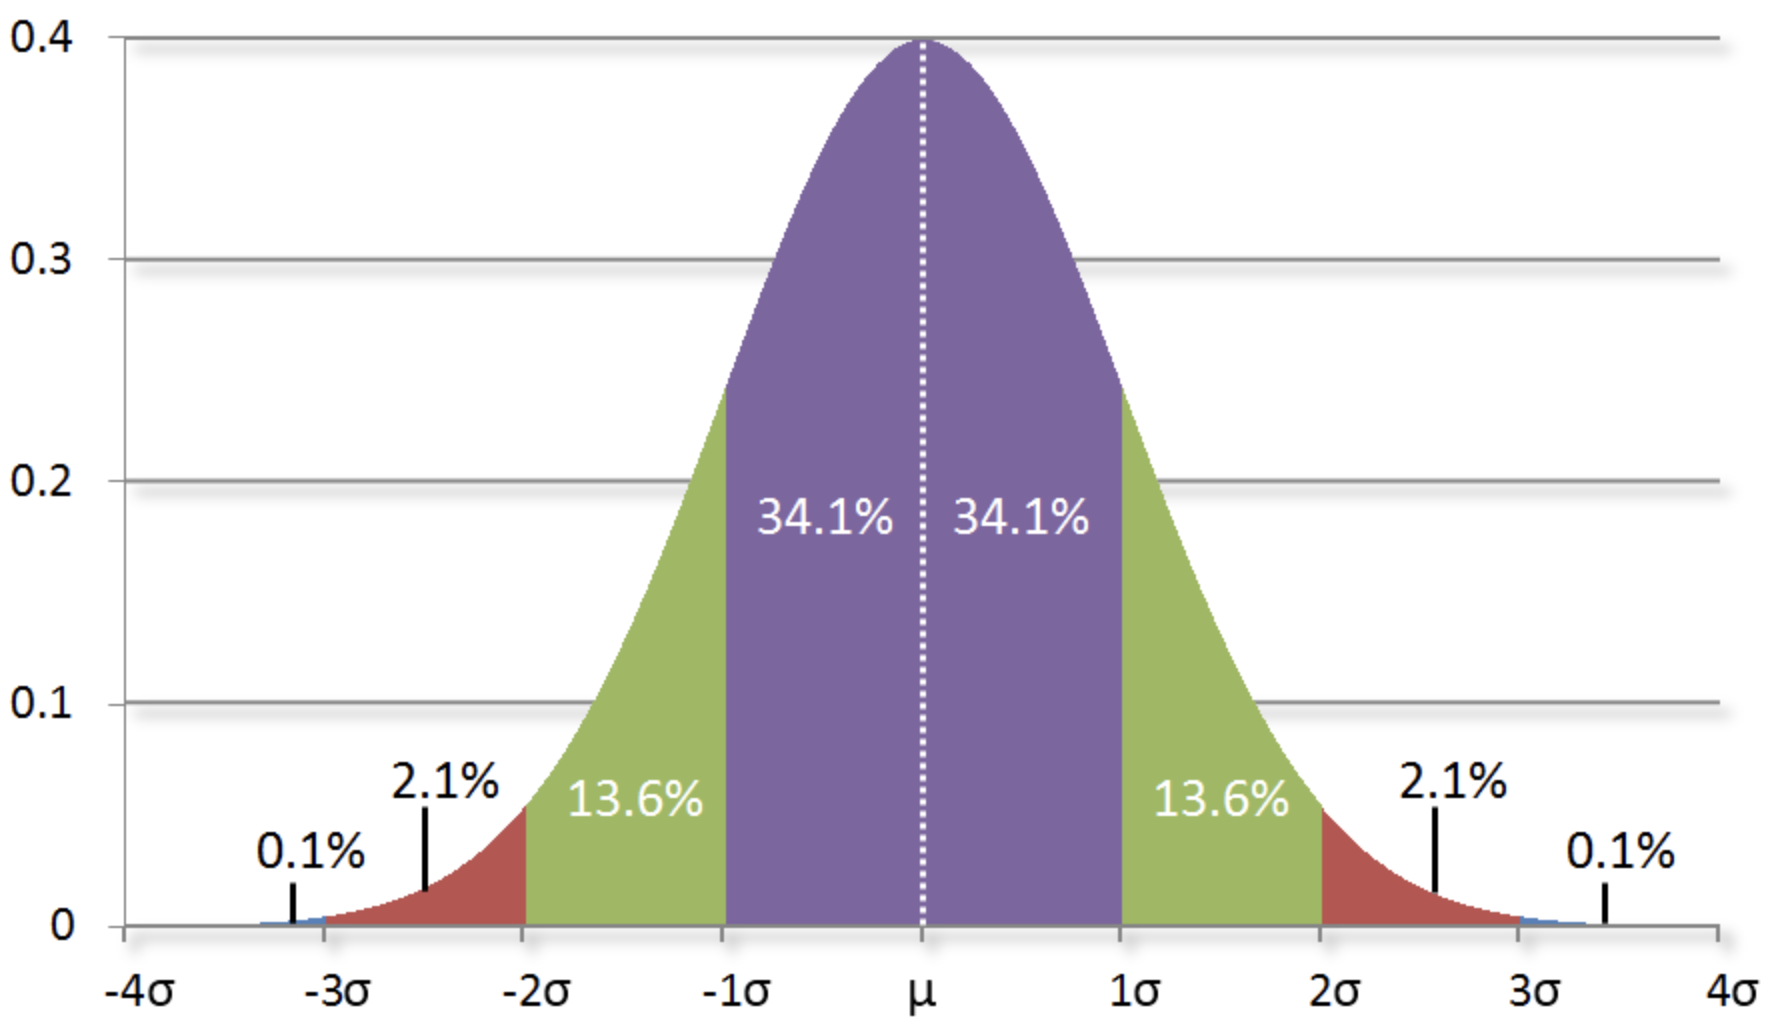
\includegraphics{../Images/Courbe_normale.png}

Quelque soit la forme de la loi normale:

\begin{enumerate}
\def\labelenumi{\arabic{enumi}.}
\item
  L'intervalle d'un écart-type de part et d'autre de la moyenne contient
  68\% de la distribution
\item
  L'intervalle de deux écart-types de part et d'autre de la moyenne
  contient 95\% de la distribution
\item
  L'intervalle de trois écart-types de part et d'autre de la moyenne
  contient 99,7\% de la distribution
\end{enumerate}

\hypertarget{ecart-type-correspondant-uxe0-x-pourcentage-de-la-distribution}{%
\subsection{Ecart-type correspondant à x pourcentage de la
distribution}\label{ecart-type-correspondant-uxe0-x-pourcentage-de-la-distribution}}

\begin{itemize}
\tightlist
\item
  Il est préférable de partir de l'intervalle de déterminer plus
  précisément le nombre d'écart-type qui délimite l'intervalle.
\end{itemize}

\begin{quote}
\begin{itemize}
\tightlist
\item
  Par exemple, quel intervalle contient 60\% de la distribution?
\end{itemize}
\end{quote}

\begin{quote}
\begin{itemize}
\tightlist
\item
  Autrement dit, comme la courbe est symétrique, on dira que 30\% de la
  distribution se trouve entre la moyenne et la valeur recherchée. Donc
  que 20\% se trouve au-delà.
\end{itemize}
\end{quote}

\begin{quote}
\begin{itemize}
\tightlist
\item
  Prob(distribution \textless{} v1) = 0.2 nous donne tout simplement la
  valeur de 20 ième percentile de la distribution
\end{itemize}
\end{quote}

\begin{quote}
\begin{itemize}
\tightlist
\item
  Prob(distribution \textless{} v2) = 0.8 dit que 80\% de la
  distribution est inférieure à cette valeur.
\end{itemize}
\end{quote}

\begin{quote}
\begin{itemize}
\tightlist
\item
  Donc l'intervalle {[}V1, V2{]} contient 60\% (80\% - 20\%) de la
  distribution
\end{itemize}
\end{quote}

\hypertarget{ecart-type-correspondant-uxe0-x-pourcentage-de-la-distribution-1}{%
\subsection{Ecart-type correspondant à x pourcentage de la
distribution}\label{ecart-type-correspondant-uxe0-x-pourcentage-de-la-distribution-1}}

On peut le calculer assez facilement avec la fonction qnorm.

\begin{Shaded}
\begin{Highlighting}[]
\NormalTok{v1 }\OtherTok{\textless{}{-}} \FunctionTok{qnorm}\NormalTok{(}\FloatTok{0.20}\NormalTok{, }\AttributeTok{mean =} \DecValTok{5}\NormalTok{, }\AttributeTok{sd =} \DecValTok{3}\NormalTok{)}
\NormalTok{v1}
\end{Highlighting}
\end{Shaded}

\begin{verbatim}
## [1] 2.475136
\end{verbatim}

\begin{Shaded}
\begin{Highlighting}[]
\NormalTok{v2 }\OtherTok{\textless{}{-}} \FunctionTok{qnorm}\NormalTok{(}\FloatTok{0.80}\NormalTok{, }\AttributeTok{mean =} \DecValTok{5}\NormalTok{, }\AttributeTok{sd =} \DecValTok{3}\NormalTok{)}
\NormalTok{v2}
\end{Highlighting}
\end{Shaded}

\begin{verbatim}
## [1] 7.524864
\end{verbatim}

\begin{quote}
\begin{itemize}
\tightlist
\item
  Ainsi, on trouve que l'intervalle en question est {[}2,47; 7,52{]}
  pour la distribution normale N(5, 3).
\end{itemize}
\end{quote}

\begin{quote}
\begin{itemize}
\tightlist
\item
  Cet intervalle contient 60\% de la distribution
\end{itemize}
\end{quote}

\hypertarget{ecart-type-correspondant-uxe0-x-pourcentage-de-la-distribution-2}{%
\subsection{Ecart-type correspondant à x pourcentage de la
distribution}\label{ecart-type-correspondant-uxe0-x-pourcentage-de-la-distribution-2}}

\begin{Shaded}
\begin{Highlighting}[]
\FunctionTok{ggplot}\NormalTok{(}\AttributeTok{data =} \FunctionTok{data.frame}\NormalTok{(}\AttributeTok{x =} \FunctionTok{c}\NormalTok{(}\SpecialCharTok{{-}}\DecValTok{5}\NormalTok{, }\DecValTok{15}\NormalTok{)), }\FunctionTok{aes}\NormalTok{(x)) }\SpecialCharTok{+}
  \FunctionTok{stat\_function}\NormalTok{(}\AttributeTok{fun =}\NormalTok{ dnorm, }\AttributeTok{args =} \FunctionTok{list}\NormalTok{(}\AttributeTok{mean =} \DecValTok{5}\NormalTok{, }\AttributeTok{sd =} \DecValTok{3}\NormalTok{), }\AttributeTok{color =} \StringTok{"red"}\NormalTok{) }\SpecialCharTok{+}
  \FunctionTok{stat\_function}\NormalTok{(}\AttributeTok{fun =}\NormalTok{ dnorm, }\AttributeTok{args =} \FunctionTok{list}\NormalTok{(}\AttributeTok{mean =} \DecValTok{5}\NormalTok{, }\AttributeTok{sd =} \DecValTok{3}\NormalTok{),}
                \AttributeTok{geom =} \StringTok{"area"}\NormalTok{, }\AttributeTok{fill =} \StringTok{"red"}\NormalTok{, }\AttributeTok{xlim =} \FunctionTok{c}\NormalTok{(v1, v2), }\AttributeTok{alpha =} \FloatTok{0.2}\NormalTok{)}
\end{Highlighting}
\end{Shaded}

\includegraphics{Seance5.3_livre_Parametres_variation_détaillé_files/figure-latex/unnamed-chunk-5-1.pdf}

\hypertarget{loi-normale-centruxe9e-ruxe9duite}{%
\subsection{Loi normale (centrée
réduite)}\label{loi-normale-centruxe9e-ruxe9duite}}

\begin{itemize}
\tightlist
\item
  Calculer les quantiles pour différentes distributions normales peut
  être fastidieux (dans le temps).
\item
  Alors, les statisticiens ont calculé cela pour la distribution normale
  centrée réduite
\item
  Lorsque la moyenne vaut 0 et l'écart-type vaut 1, on parle de
  distribution normale centrée réduite
\item
  Vous comprenez donc que si vous standardisez les scores de votre
  distribution normale, vous trouvez une distribution normale centrée
  réduite
\end{itemize}

\hypertarget{loi-normale-centruxe9e-ruxe9duite-1}{%
\subsection{Loi normale (centrée
réduite)}\label{loi-normale-centruxe9e-ruxe9duite-1}}

\begin{Shaded}
\begin{Highlighting}[]
\NormalTok{courbe\_normale }\OtherTok{\textless{}{-}} 
  \FunctionTok{ggplot}\NormalTok{(}\AttributeTok{data =} \FunctionTok{data.frame}\NormalTok{(}\AttributeTok{x =} \FunctionTok{c}\NormalTok{(}\SpecialCharTok{{-}}\DecValTok{4}\NormalTok{, }\DecValTok{4}\NormalTok{)), }\FunctionTok{aes}\NormalTok{(x)) }\SpecialCharTok{+}
  \FunctionTok{stat\_function}\NormalTok{(}\AttributeTok{fun =}\NormalTok{ dnorm, }\AttributeTok{args =} \FunctionTok{list}\NormalTok{(}\AttributeTok{mean =} \DecValTok{0}\NormalTok{, }\AttributeTok{sd =} \DecValTok{1}\NormalTok{), }\AttributeTok{color =} \StringTok{"blue"}\NormalTok{) }

\NormalTok{courbe\_normale}
\end{Highlighting}
\end{Shaded}

\includegraphics{Seance5.3_livre_Parametres_variation_détaillé_files/figure-latex/unnamed-chunk-6-1.pdf}

\begin{Shaded}
\begin{Highlighting}[]
\NormalTok{?dnorm}
\end{Highlighting}
\end{Shaded}

\hypertarget{loi-normale-centruxe9e-ruxe9duite-2}{%
\subsection{Loi normale (centrée
réduite)}\label{loi-normale-centruxe9e-ruxe9duite-2}}

\includegraphics{Seance5.3_livre_Parametres_variation_détaillé_files/figure-latex/unnamed-chunk-7-1.pdf}

\begin{itemize}
\tightlist
\item
  On voit que 68\% de la distribution est comprise entre -1 et 1
  écart-type (vert foncé)
\item
  On voit que 95\% de la distribution est comprise entre -2 (-1.96) et 2
  (1.96) écarts-types (vert clair)
\end{itemize}

\hypertarget{lecture-du-tableau-de-distribution}{%
\subsection{Lecture du tableau de
distribution}\label{lecture-du-tableau-de-distribution}}

Voir livre

\hypertarget{distribution-duxe9chantillonnage}{%
\section{Distribution
d'échantillonnage}\label{distribution-duxe9chantillonnage}}

\hypertarget{distribution-duxe9chantillonnage-1}{%
\subsection{Distribution
d'échantillonnage}\label{distribution-duxe9chantillonnage-1}}

\begin{itemize}
\item
  Il est possible d'utiliser des distributions de données d'échantillon
  afin de décrire la population de laquelle fut tiré l'échantillon
\item
  Une \textbf{distribution d'échantillonnage} (par exemple de la
  moyenne) est la distribution de l'ensemble des moyennes calculées sur
  l'ensemble des échantillons possibles de taille N qu'on peut tirer de
  cet échantillon
\end{itemize}

\hypertarget{distribution-duxe9chantillonnage-2}{%
\subsection{Distribution
d'échantillonnage}\label{distribution-duxe9chantillonnage-2}}

\begin{itemize}
\item
  Exemple simple

  \begin{itemize}
  \tightlist
  \item
    Voici les âges de 4 personnes \{10, 11, 13, 14\}
  \item
    Voici les échantillons possibles de 3 personnes qu'on peut tirer de
    cette population:
  \end{itemize}
\end{itemize}

\begin{quote}
\begin{itemize}
\tightlist
\item
  (10, 11, 13) avec la moyenne de 11,3 ans
\item
  (10, 11, 14) avec la moyenne de 11,7 ans
\item
  (11, 13, 14) avec la moyenne de 12,7 ans
\end{itemize}
\end{quote}

\begin{quote}
\begin{itemize}
\tightlist
\item
  11,3; 11,7 et 12,7 est appellé la distribution d'échantillonnage
\end{itemize}
\end{quote}

\hypertarget{distribution-duxe9chantillonnage-3}{%
\subsection{Distribution
d'échantillonnage}\label{distribution-duxe9chantillonnage-3}}

\url{https://www.alloprof.qc.ca/fr/eleves/bv/mathematiques/les-permutations-les-arrangements-et-les-combinai-m1346}

\begin{itemize}
\item
  Exemple simple
\item
  Voici les âges de 4 personnes \{10, 11, 13, 14\}
\item
  Tirage sans remise de 3 personnes parmi 4: 4!/(4-3)!x3! = 4
\item
  Tirage avec remise : (4+3-1)!/(4-3)!x3! = 6!/1!x3! = 120
\end{itemize}

\hypertarget{distribution-duxe9chantillonnage---propriuxe9tuxe9}{%
\subsection{Distribution d'échantillonnage -
propriété}\label{distribution-duxe9chantillonnage---propriuxe9tuxe9}}

\begin{itemize}
\tightlist
\item
  A mesure qu'augmente la taille N de l'échantillon, la distribution
  d'échantillonnage de la moyenne s'apparente de plus en plus à une
  distribution normale, dont la moyenne est semblable à celle de la
  \textbf{population} et dont l'écart-type est de
  \(\frac{\sigma}{\sqrt{N}}\)
\end{itemize}

\begin{quote}
\begin{itemize}
\tightlist
\item
  On nomme cela le \textbf{théorème de limite centrale}
\end{itemize}
\end{quote}

\begin{quote}
\begin{itemize}
\tightlist
\item
  L'écart-type de la distribution d'échantillonnage est appelé
  \textbf{erreur-type}
\end{itemize}
\end{quote}

\begin{quote}
\begin{itemize}
\tightlist
\item
  Il vaut: \(\frac{\sigma}{\sqrt{N}}\)
\end{itemize}
\end{quote}

\hypertarget{exemple}{%
\subsection{Exemple}\label{exemple}}

\begin{itemize}
\tightlist
\item
  Supposons que le salaire moyen issu d'un échantillon de 1000 Québécois
  vaut 65000\$ et l'écart-type de 32000.
\end{itemize}

\begin{quote}
\begin{itemize}
\tightlist
\item
  On dira que le salaire moyen des Québécois vaut 65000\$. Mais, ce
  faisant on commet une ereur.
\end{itemize}
\end{quote}

\begin{quote}
\begin{itemize}
\tightlist
\item
  Si nous approximons aussi l'écart-type du salaire de la population par
  l'écart-type du salaire de l'échantillon, on peut alors dire que
  l'erreur-type vaut:
\end{itemize}
\end{quote}

\begin{quote}
\begin{itemize}
\tightlist
\item
  32000/racine\_carré (1000) = 1012
\end{itemize}
\end{quote}

\hypertarget{intervalle-de-confiance}{%
\section{Intervalle de confiance}\label{intervalle-de-confiance}}

\hypertarget{intervalle-de-confiance-1}{%
\subsection{Intervalle de confiance}\label{intervalle-de-confiance-1}}

\begin{itemize}
\tightlist
\item
  La meilleure estimation que nous pouvons avoir de la moyenne de la
  population est la moyenne de l'échantillon
\end{itemize}

\begin{quote}
\begin{itemize}
\tightlist
\item
  Cependant, cette moyenne calculée à partir d'un seul échantillon peut
  être soit plus élevée, ou plus faible que la vraie moyenne de la
  population
\end{itemize}
\end{quote}

\begin{quote}
\begin{itemize}
\tightlist
\item
  Il parait donc extrêmement utile de déterminer l'intervalle, de part
  et d'autre de la moyenne, à l'intérieur duquel il est probable de
  trouver la moyenne de la population
\end{itemize}
\end{quote}

\begin{quote}
\begin{itemize}
\tightlist
\item
  L'erreur-type va nous aider à trouver cela
\end{itemize}
\end{quote}

\hypertarget{intervalle-de-confiance-2}{%
\subsection{Intervalle de confiance}\label{intervalle-de-confiance-2}}

Le théorème de la limite centrale nous permet de déterminer cette
intervalle.

\begin{quote}
\begin{itemize}
\tightlist
\item
  On sait que plus N est grand, plus la distribution d'échantillonnge va
  suivre la distribution normale N(moyenne de l'échantillon,
  \(\sigma/\sqrt(N)\))
\end{itemize}
\end{quote}

\begin{quote}
\begin{itemize}
\tightlist
\item
  On sait aussi que dans une distribution normale, 95\% de la
  distribution se trouve à plus ou moins 2 écart-types de la moyenne
  (plus précisément à 1.96 écart-type)
\end{itemize}
\end{quote}

\begin{quote}
\begin{itemize}
\tightlist
\item
  Ainsi, l'intervalle de confiance à 95\% sera déterminée par:
\end{itemize}
\end{quote}

\hypertarget{intervalle-de-confiance-3}{%
\subsection{Intervalle de confiance}\label{intervalle-de-confiance-3}}

\[ [\bar{X} - 1.96\sigma_{\bar{X}} , \bar{X} + 1.96\sigma_{\bar{X}}]\]

\begin{quote}
\begin{itemize}
\tightlist
\item
  Dans l'exemple précédent, on dira que dans 95\% des cas, le salaire
  moyen de la population Québécoise va se trouver dans l'intervalle
  {[}65000 - 1.96x1012, 65000 + 1.96x1012{]}, soit {[}63016, 66983{]}
\end{itemize}
\end{quote}

\begin{quote}
\begin{itemize}
\tightlist
\item
  1,96 est la valeur du score standardisé correspondant à l'intervalle
  de 95\%
\end{itemize}
\end{quote}

\hypertarget{thuxe9oruxe8me-central-limite---ruxe8gle-de-lapproximation-normale-guxe9nuxe9ralituxe9}{%
\section{Théorème central limite - Règle de l'Approximation Normale
(généralité)}\label{thuxe9oruxe8me-central-limite---ruxe8gle-de-lapproximation-normale-guxe9nuxe9ralituxe9}}

\hypertarget{duxe9gruxe9-de-fiabilituxe9-de-luxe9chantillon}{%
\subsection{Dégré de fiabilité de
l'échantillon}\label{duxe9gruxe9-de-fiabilituxe9-de-luxe9chantillon}}

\begin{itemize}
\item
  Le but de l'échantillonnage aléatoire est d'éffectuer une inférence
  relative à la population sous-jacente.
\item
  On souhaite que la moyenne de l'échantillon - \(\bar{X}\) soit une
  estimation proche de la moyenne de la population - \(\mu\).
\item
  Deux façons d'étudier le degré d'approximation de \(\mu\) par
  \(\bar{X}\).
\end{itemize}

\begin{enumerate}
\def\labelenumi{\arabic{enumi}.}
\tightlist
\item
  A partir de formules mathématiques
\item
  A partir de la distribution d'échantillonnage
\end{enumerate}

\hypertarget{moments-de-la-moyenne-de-luxe9chantillon}{%
\subsection{Moments de la moyenne de
l'échantillon}\label{moments-de-la-moyenne-de-luxe9chantillon}}

\begin{itemize}
\item
  On démontre que :
\item
  E(\(\bar{X}\)) = \(\mu\) : la moyenne de l'échantillonnage \(\bar{X}\)
  coïncidera en moyenne avec l'objectif, ie. \(\bar{X}\) égalisera
  \(\mu\)
\item
  Erreur type d'échantillon (standard error) = SE = \(\sigma_{\bar{X}}\)
  = \(\frac{\sigma}{\sqrt{n}}\), où \(\sigma\) est l'écart type dans la
  population
\item
  L'erreur type de \(\bar{X}\) diminue quand la taille de l'échantillon
  aléatoire augmente.
\item
  Plus l'échantillon est grand, plus \(\bar{X}\) donne une estimation
  exacte de la moyenne de la population.
\item
  \textbf{NB}: Ne pas confondre:
\item
  écart type (en anglais, standard deviation) et
\item
  erreur type ou écart type d'échantillon (en anglais, standard error)
\end{itemize}

\hypertarget{forme-de-la-distribution-duxe9chantillonnage}{%
\subsection{Forme de la distribution
d'échantillonnage}\label{forme-de-la-distribution-duxe9chantillonnage}}

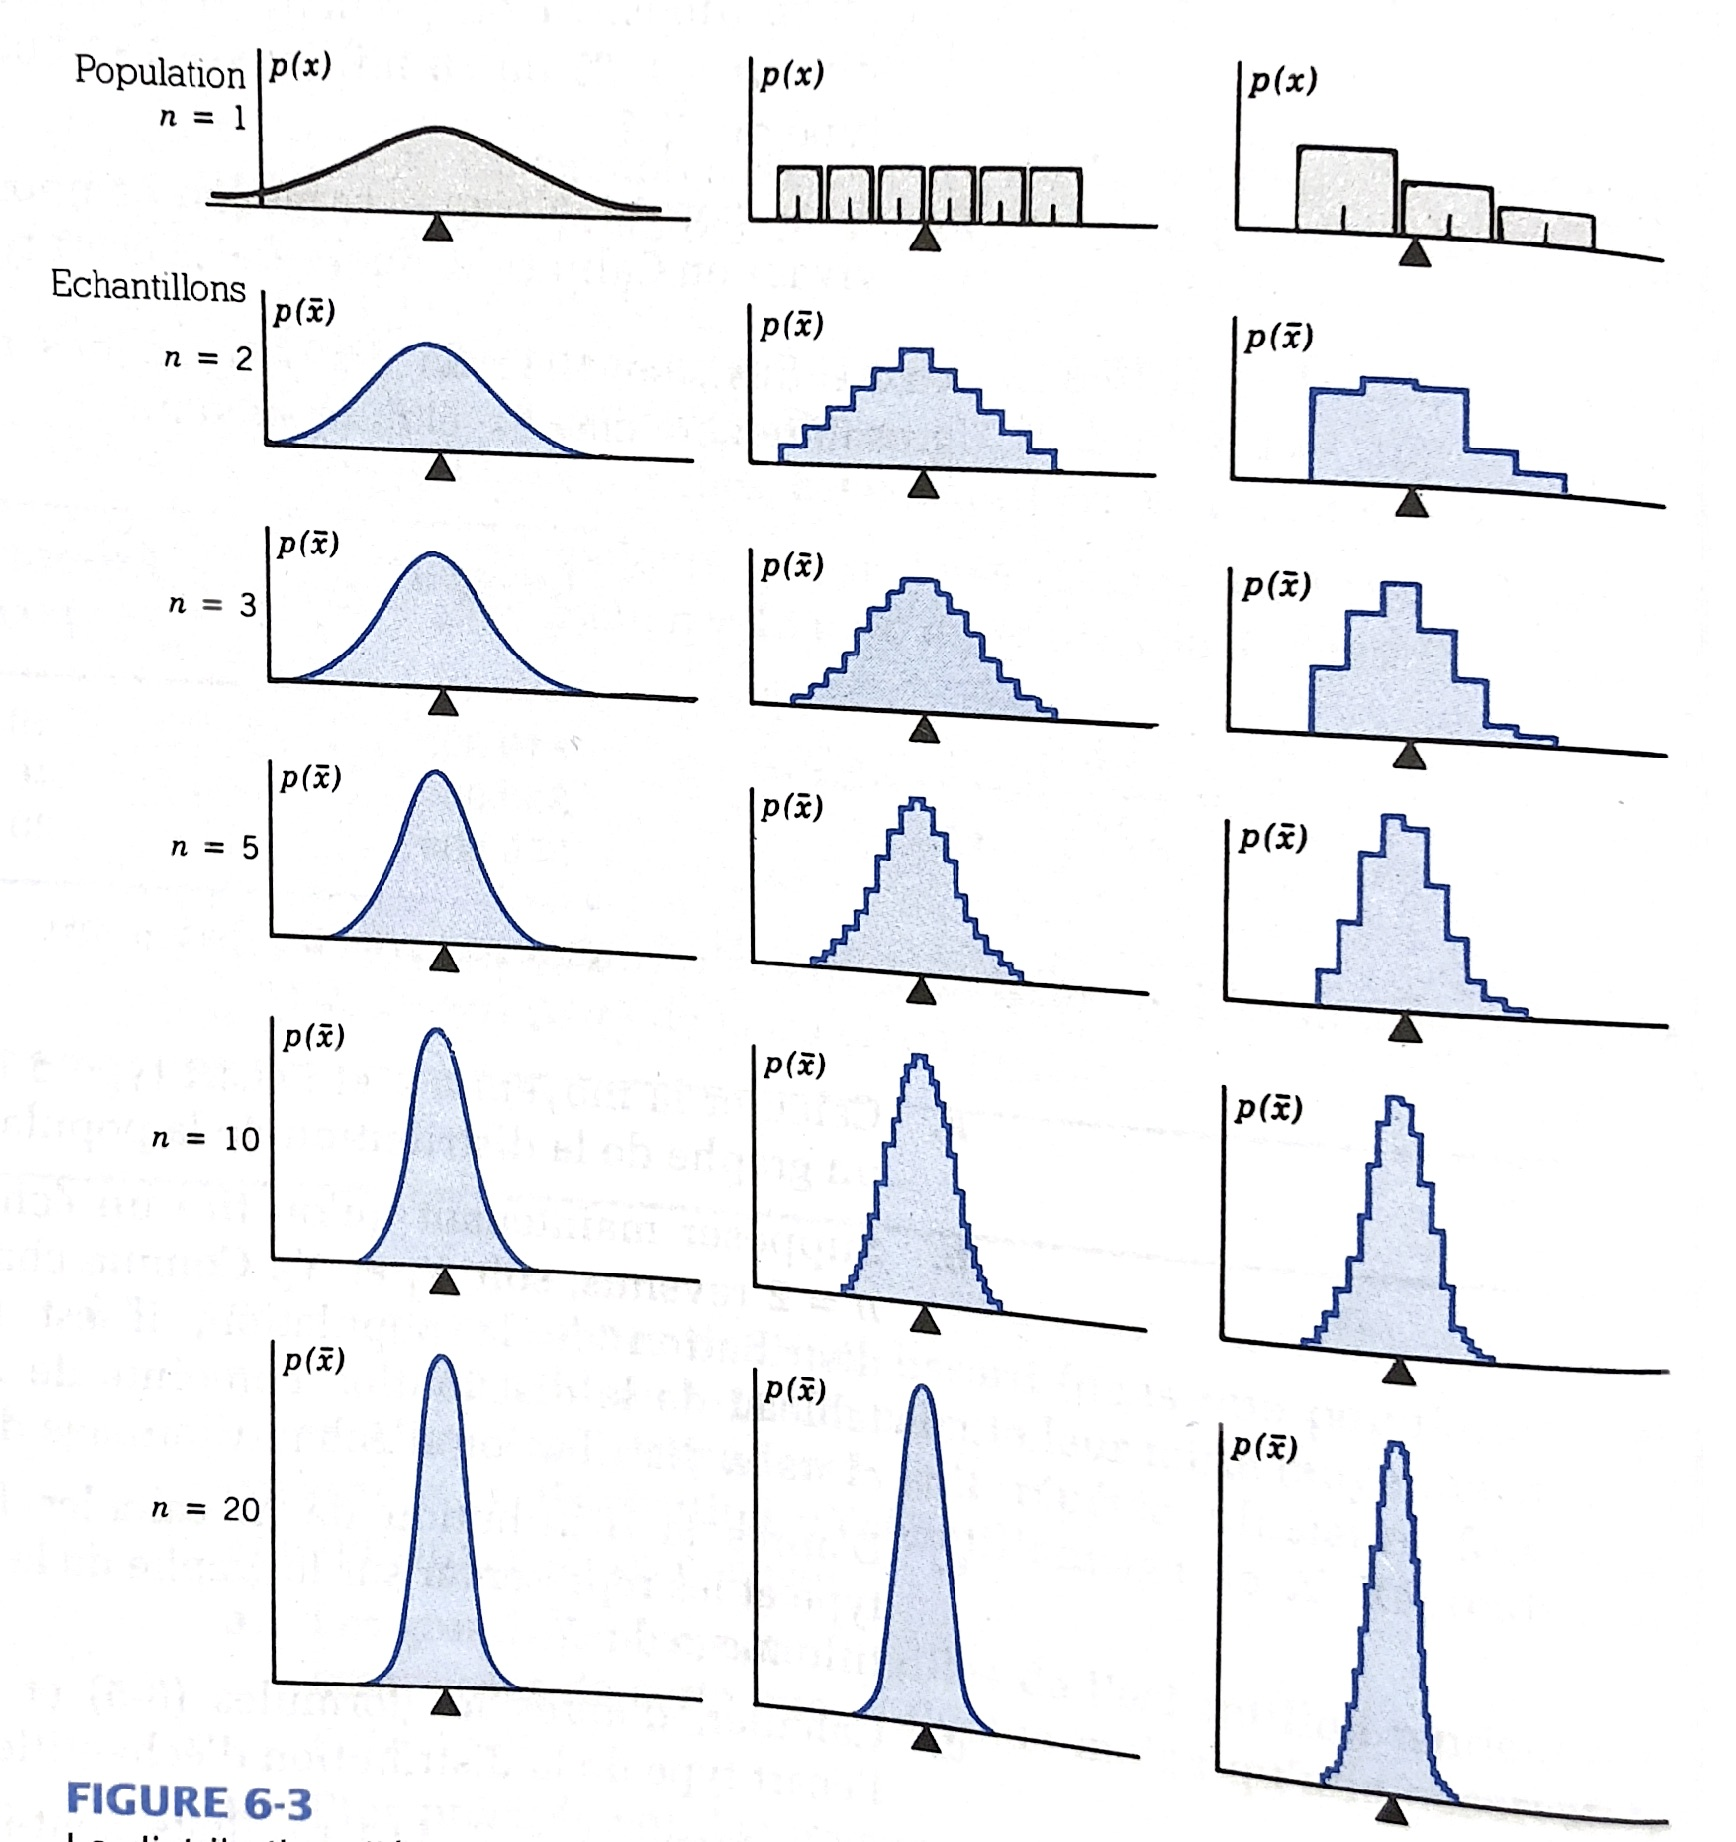
\includegraphics{../Images/distribution_echantillonnage.jpg}

\hypertarget{thuxe9oruxe8me-central-limite-ruxe8gle-de-lapproximation-normale}{%
\subsection{Théorème central limite (Règle de l'Approximation
Normale)}\label{thuxe9oruxe8me-central-limite-ruxe8gle-de-lapproximation-normale}}

Dans les échantillons aléatoires de taille n, la moyenne de
l'échantillon \(\bar{X}\) varie autour de la moyenne de la population
\(\mu\) avec un écart type égal à \(\frac{\sigma}{\sqrt{n}}\) (ou
\(\sigma\) est l'écart type de la population). Donc, quand n s'accroît,
la distribution d'échantillonnage de \(\bar{X}\) est de plus en plus
concentrée autour de son objectif \(\mu\). Elle devient de plus en plus
proche de la distribution normale (forme de cloche).

\hypertarget{thuxe9oruxe8me-central-limite-ruxe8gle-de-lapproximation-normale-1}{%
\subsection{Théorème central limite (Règle de l'Approximation
Normale)}\label{thuxe9oruxe8me-central-limite-ruxe8gle-de-lapproximation-normale-1}}

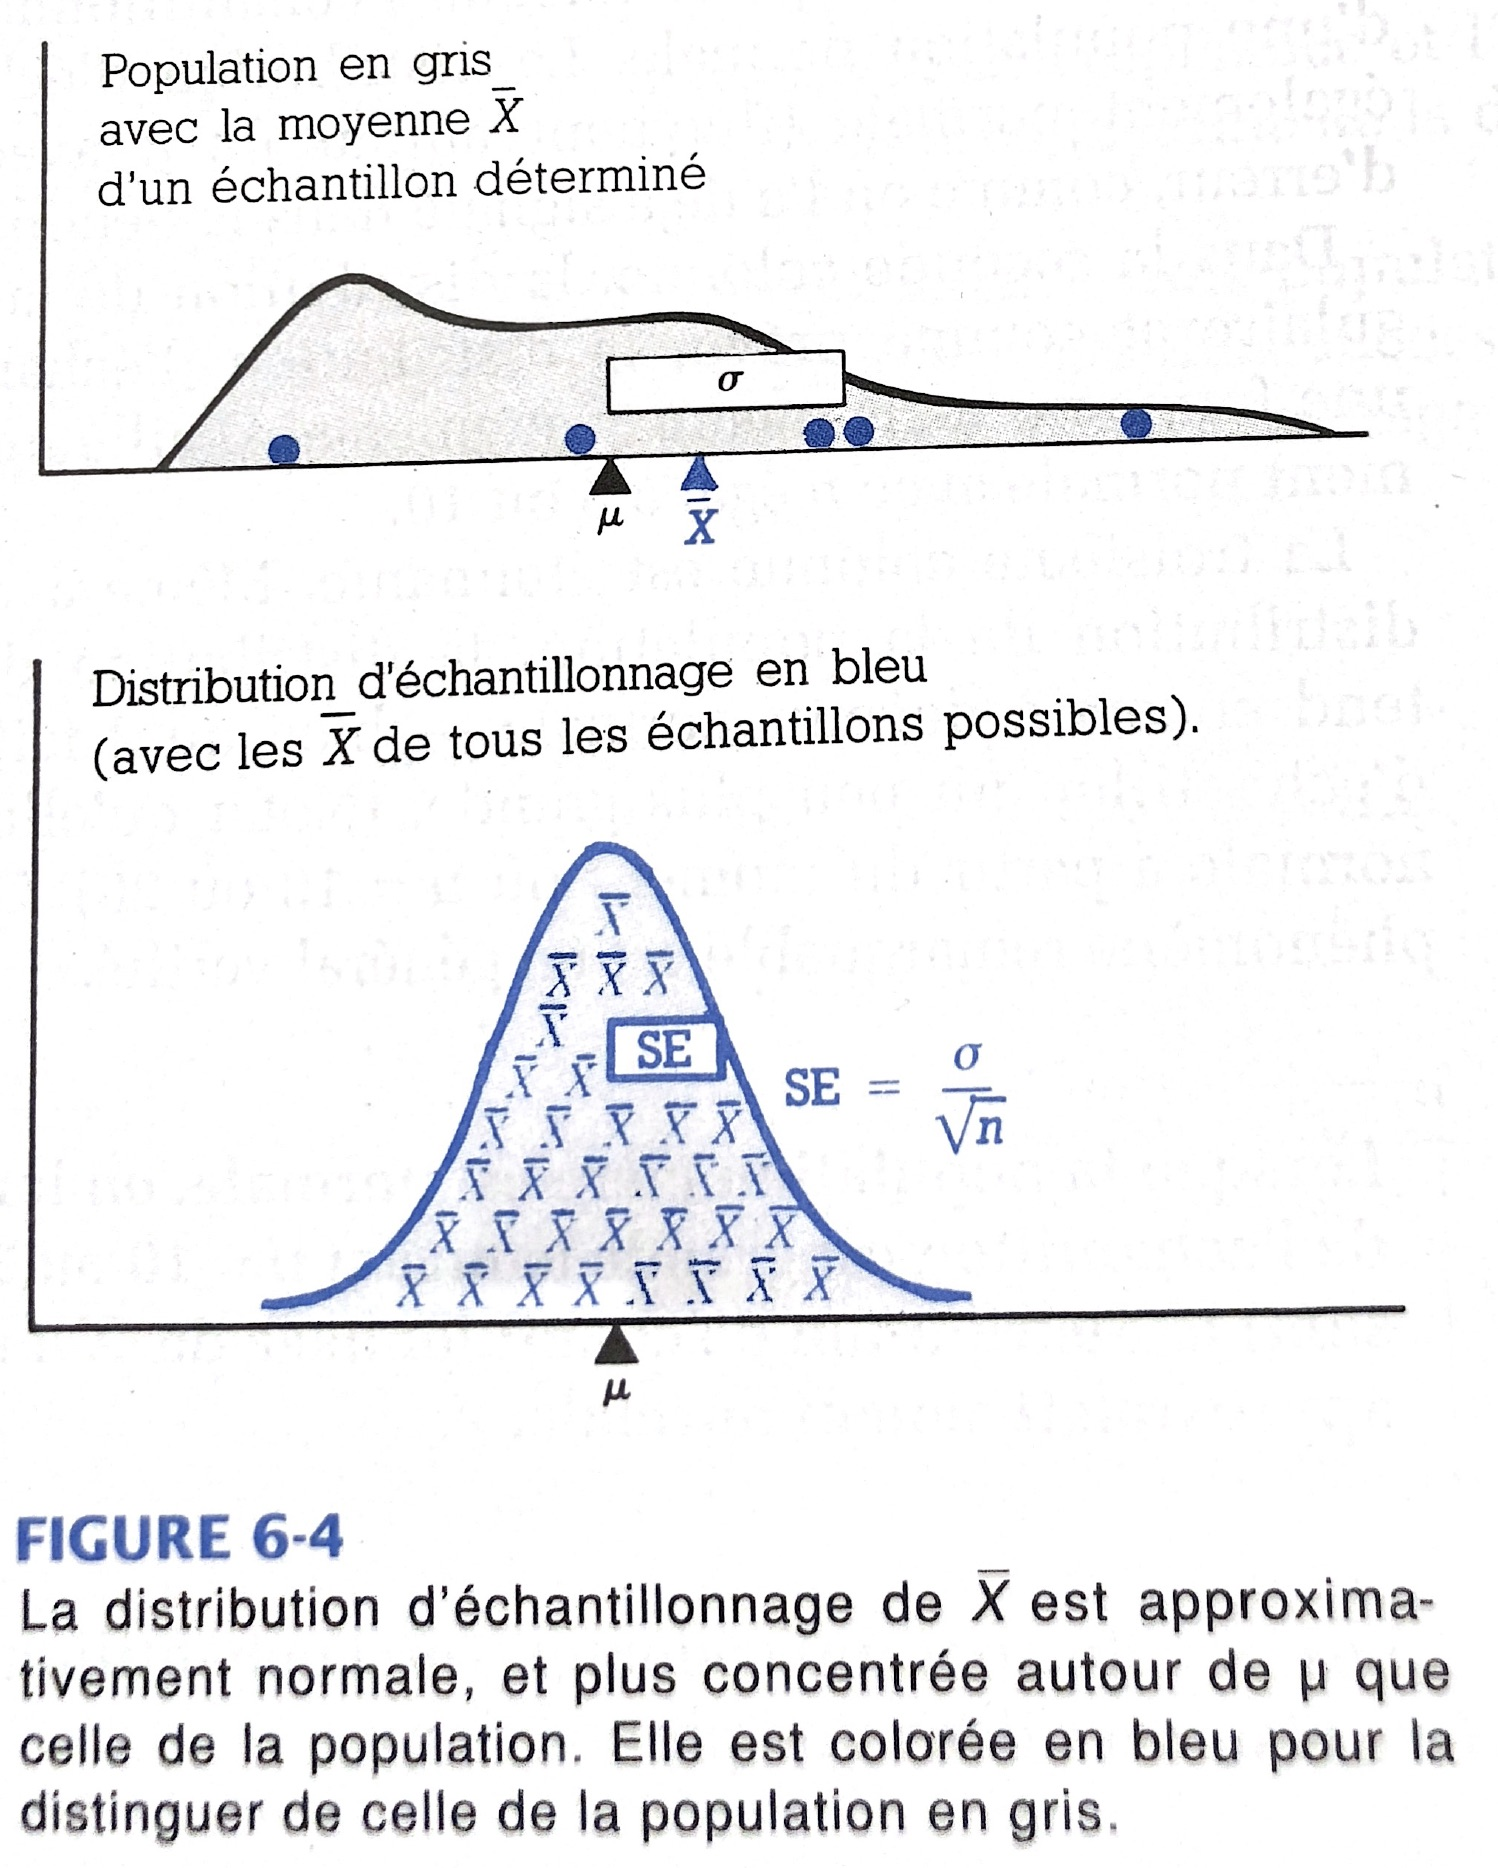
\includegraphics{../Images/tcl.jpg}

\hypertarget{thuxe9oruxe8me-de-la-limite-centrale-ruxe8gle-de-lapproximation-normale}{%
\subsection{Théorème de la limite centrale (Règle de l'Approximation
Normale)}\label{thuxe9oruxe8me-de-la-limite-centrale-ruxe8gle-de-lapproximation-normale}}

\begin{itemize}
\item
  Dire que la moyenne de l'échantillon \(\bar{X}\) varie autour de la
  moyenne de la population \(\mu\) avec une erreur type
  \(\sigma_{\bar{X}}\) égale à \(\frac{\sigma}{\sqrt{n}}\) revient à
  dire que la distribution \(\bar{X}\) suit une loi normale de moyenne
  \(\mu\) et d'écart type \(\frac{\sigma}{\sqrt{n}}\)
\item
  \(\bar{X}\) suit \(N(\mu, \frac{\sigma}{\sqrt{n}})\)
\item
  Ou que (\(\frac{(\bar{X}-\mu)}{\frac{\sigma}{\sqrt{n}}}\)) suit une
  loi \textbf{normale dite centrée réduite} N(0,1)
\end{itemize}

\hypertarget{thuxe9oruxe8me-de-la-limite-centrale-ruxe8gle-de-lapproximation-normale---exemple}{%
\subsection{Théorème de la limite centrale (Règle de l'Approximation
Normale) -
Exemple}\label{thuxe9oruxe8me-de-la-limite-centrale-ruxe8gle-de-lapproximation-normale---exemple}}

Une population d'étudiants d'un grand campus du Middle-West a une taille
moyenne de \(\mu\) = 175.26 cm (69 inches) et un écart type \(\sigma\) =
8.18cm (3.22 inches). Si un échantillon aléatoire de n = 10 individus
est prélevé, quelle est la probabilité pour que la moyenne de
l'échantillon \(\bar{X}\) s'écarte de 5.08 cm (2 inches) de la moyenne
de la population?

\begin{verbatim}
## [1] 1.018253
\end{verbatim}

\includegraphics{Seance5.3_livre_Parametres_variation_détaillé_files/figure-latex/unnamed-chunk-8-1.pdf}

\hypertarget{thuxe9oruxe8me-central-limite-ruxe8gle-de-lapproximation-normale---exemple}{%
\subsection{Théorème central limite (Règle de l'Approximation Normale) -
Exemple}\label{thuxe9oruxe8me-central-limite-ruxe8gle-de-lapproximation-normale---exemple}}

\begin{itemize}
\item
  \textbf{Réponse}:
\item
  Selon la Règle de l'Approximation Normale, \(\bar{X}\) est normalement
  distribuée avec:
\item
  Espérance = \(\mu\) = 69 et
\item
  Écart type d'échantillon =
  \(\sigma_{\bar{X}} = \frac{\sigma}{\sqrt{n}} = \frac{3.22}{\sqrt{10}}\)
  = 1.02
\item
  On cherche à déterminer la probabilité que \(\bar{X}\) s'écarte de 2
  inches de \(\mu\), c'est à dire qu'elle se trouve entre 67 et 71.
\item
  Aussi, calcule-t-on, d'abord la probabilité que \(\bar{X}\) soit
  supérieur à 71, en commençant par centrer et réduire:
\end{itemize}

\[\text{Z = } \frac{\bar{X}-\mu}{\sigma_{\bar{X}}} = \frac{71 - 69}{1.02} = 1.96\]

\begin{itemize}
\tightlist
\item
  Cela signifie que la valeur critique de 71 pour que la moyenne de
  l'échantillon est environ de 2 écarts-type au dessus de son espérance
  69.
\end{itemize}

\hypertarget{thuxe9oruxe8me-central-limite-ruxe8gle-de-lapproximation-normale---exemple-1}{%
\subsection{Théorème central limite (Règle de l'Approximation Normale) -
Exemple}\label{thuxe9oruxe8me-central-limite-ruxe8gle-de-lapproximation-normale---exemple-1}}

\begin{itemize}
\tightlist
\item
  D'après le tableau de la loi normale centrée réduite, on trouve que la
  probabilité que Z excède 1.96 est seulement de 0.025. C'est ce que
  montre la partie droite hachurée sur la figure (montrer la figure en
  classe).
\item
  En raison de la symétrie de la distribution normale, l'extrémité
  gauche a la même probabilité 0.025.
\item
  Ainsi, on peut déterminer la probabilité cherchée de la partie
  centrale : \(Probabilité = 1.000 - 0.025 - 0.025 = 0.95\)
\item
  On conclut donc qu'il y a 95\% de chance pour que la moyenne de
  l'échantillon s'écarte de 2 inches de la moyenne de la population
\end{itemize}

\hypertarget{thuxe9oruxe8me-central-limite-ruxe8gle-de-lapproximation-normale---question}{%
\subsection{Théorème central limite (Règle de l'Approximation Normale) -
Question}\label{thuxe9oruxe8me-central-limite-ruxe8gle-de-lapproximation-normale---question}}

\begin{enumerate}
\def\labelenumi{\arabic{enumi}.}
\tightlist
\item
  Quelle est la probabilité que cette moyenne s'écarte de 1 inche de la
  moyenne de la population? Est-ce que cette probabilité va être plus
  grande ou plus pétite que la première?
\item
  Quelle est la probabilité que cette moyenne s'écarte de 3 inches de la
  moyenne de la population? Est-ce que cette probabilité va être plus
  grande ou plus pétite que la première?
\end{enumerate}

\end{document}
